\documentclass[a4paper,twocolumn,12pt]{article}
\usepackage[left=1.5cm, right=1.5cm, top=2cm,bottom=2cm]{geometry}
\usepackage{amsmath, amssymb, amsfonts}
\usepackage{enumerate}
\usepackage{graphicx}
\usepackage{tikz}
\begin{document} 
\section*{Piape Matemática} 
 
\subsection*{Módulo I}
\subsection*{Exercícios Aula 02}
   
\paragraph*{1.} Para cada descrição abaixo, enumere os elementos dos conjuntos envolvidos e represente-os em diagramas de Venn.

\begin{enumerate}[a)]
\item  \(A\) é o conjunto dos números pares entre 1 e 20.
\item \(B\) é o conjunto dos números ímpares entre 1 e 20.
\item \(C\) é o conjunto dos números primos entre 1 e 20.
\item \(D\) é o conjunto dos números múltiplos de 3 entre 1 e 20.
\item \(E\) é o conjunto dos números múltiplos de 5 entre 1 e 20.
\item \(F\) é o conjunto dos números primos que são pares. 
\item \(G\) é o conjunto dos números múltiplos de 6 entre 1 e 20.
\end{enumerate}

\paragraph*{2.} Considerando os conjuntos da questão anterior, complete os itens abaixo utilizando os símbolos \(\in\) e \(\notin\), \(\subseteq\) e \(\not\subseteq\).

\medskip
\newcommand{\complete}{\underline{\hspace{7mm}} }

\begin{minipage}[t]{0.4\columnwidth}
  
\begin{enumerate}[a)]
  \item 5 \complete $A$
  \item 7 \complete $B$
  \item 2 \complete $C$
  \item 9 \complete $D$
  \item 8 \complete $E$
  \end{enumerate}
  
\end{minipage}\hfil\begin{minipage}[t]{0.3\columnwidth}

\begin{enumerate}[a)]
  \setcounter{enumi}{5}
  \item $B$ \complete $A$
  \item $D$ \complete $B$
  \item $F$ \complete $C$
  \item $G$ \complete $D$
  \item $G$ \complete $A$
  \end{enumerate}
  
\end{minipage}

\newpage

\paragraph*{3.} Se \(A\) está contido em \(B\) e \(B\) está contido em \(C\), qual
  relação podemos estabelecer entre \(A\) e \(C\)?

  \begin{enumerate}[a)]
  \item  Represente a descoberta acima usando notação simbólica.
  \item  Represente a descoberta acima usando diagramas de Venn.
  \end{enumerate}
 

\vspace*{\fill}

{\footnotesize
\paragraph*{Gabarito} \hspace*{\fill}\\
\textbf{1.} a) A = \{2, 4, 6, 8, 10, 12, 14, 16, 18, 20\}; b) B = \{1, 3, 5, 7, 9, 11, 13, 15, 17, 19\}; c) C = \{2, 3, 5, 7, 11, 13, 17, 19\}; d) D = \{3, 6, 9, 12, 15, 18\}; e) E = \{5, 10, 15, 20\}; f) F = \{2\}; g) G = \{6, 12 ,18\}\\
\textbf{2.} a) \(5\notin A\); b) \(7\in B\); c) \(2\in C\); d) \(9\in D\); e) \(8\notin E\); f) \(B\not\subseteq A\); g) \(D\not\subseteq B\); h) \(F\subseteq C\); i) \(G\subseteq D\); j) \(G\subseteq A\)\\
\textbf{3.} a) \(A \subseteq C\); b) 

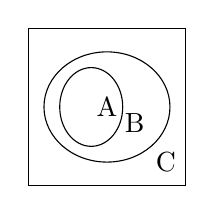
\begin{tikzpicture} 
  \draw (-0.2,0) ellipse (0.4cm and 0.5cm);
  \node at (0,0) {A};  

  \draw (0,0) ellipse (0.8cm and 0.7cm);
  \node[left] at (0.6,-0.2) {B};
  
  \draw (-1,-1) rectangle (1,1);
  \node[left] at (1,-0.7) {C};
\end{tikzpicture}

}


\end{document}